\chapter{Development Analysis}
\section{Literature Review}
Research post component selection was completed largely using the provided \gls{ti} documentation for the specific device.
\subsection{Intelligent Stepper Motor Driver with DRV8811/18/24/25}
This document is provided as a supplement to the DRV8811/18/21/24/25 data sheets. 
It provided an analogous solution for comparison to the algorithms developed on C2000 platform.
It details a technique to improve real time control of an internal indexer bipolar stepper motor driver such as the DRV8825 while obtaining programmable acceleration and deceleration profiles, speed control and position control by the utilization of a conventional MSP430 microcontroller and any of the aforementioned power stages.\cite{dev_intelligent}

\subsection{Programming TMS320x28xx and 28xxx Peripherals in C/C++}
This application report explores a hardware abstraction layer implementation to make C/C++ coding easier on C28x devices. 
This method is compared to traditional \#define macros and topics of code efficiency and special case registers are also addressed.\cite{dev_peripherals}
It was used to solve issues related to the analog GPIO systems present on the C2000, and increase over all system efficiency.

\subsection{TMS320C28x Optimizing C/C++ Compiler v6.2.4}
This user's guide discusses the characteristics of the C/C++ compiler.
It provides an overview of these tools and introduces the features of the optimizing C/C++ compiler. 
The assembler and linker are also discussed in detail.\cite{dev_optimize}
It was used for researching new compiler optimizations referenced in the Programming TMS320x28xx and 28xxx Peripherals in C/C++ documentation.

%other people can post their docs.

\section{Concept Generation}
Figure ~\ref{fig:architecture} shows the overall architecture of the Senior Thesis Project, which is fully specified by Table ~\ref{table:zerolevel}.

\begin{figure}[h]
	\centering
	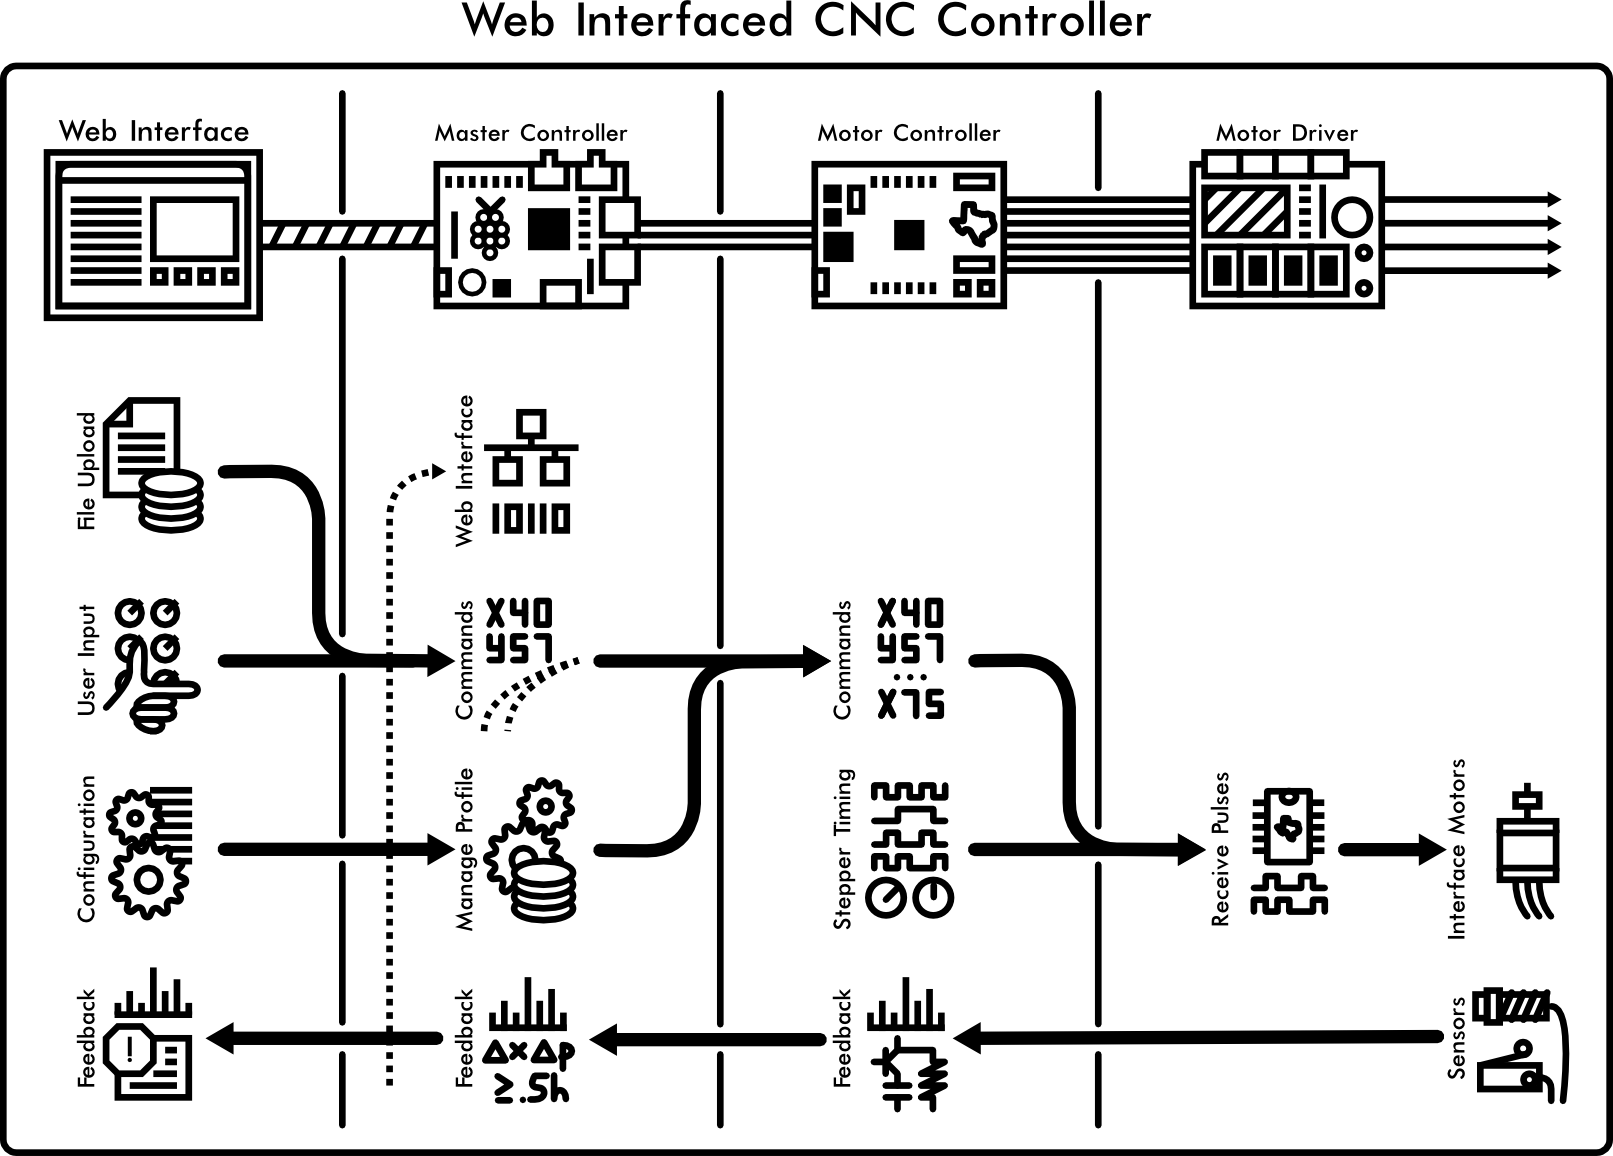
\includegraphics[width=1\textwidth]{architecture.png}
	\caption{System Architecture}
	\label{fig:architecture}
\end{figure}

\section{Concept Reduction}
\section{Production Schedule}
The CeeNC's first plan iteration started as a large reaching product.
After being advise to reduce the scope of the project, the idea for designing and developing just the control interface was decided upon.
At the same time, the main objectives, the gls{PSSC}s, were initially written.
From this point, a plan was formulated.
A gls{WBS} was designed to break each part of the project into smaller tasks.
Task dependencies were also set up using the gls{WBS}. 
From here, a gls{LRC} was designed to assign responsibility of a task to a developer.
The gls{LRC} and gls{WBS} were then used to put together an gls{AON} chart.
This gls{AON} allowed for a critical path to be determined. 
The critical path is the series of tasks that will take the longest amount of time.
Once dependencies and responsibilities were decided, a realistic schedule could be designed.
This schedule was represented in a Gantt Chart.
This Gantt Chart did go through a few iterations of design before the final schedule was set.

Once the schedule was set, the implementation phase of the project started. 
Each member worked on assigned tasks individually or with other members if it was needed.
The project stayed on schedule most of the time.
The progress of the project was tracked in each member's log books, an online tracker, and an gls{OPPM}.
The gls{OPPM} is a document that compiles all the information from the gls{WBS}, gls{LRC}, Gantt Chart, and budget onto one page to give to upper management.
Each week, a team meeting was held where updates would be given to make sure that tasks were getting done and to plan the next week's work.
This would also be reflected on the gls{OPPM}.

One recommendation for the next plan would be to include more time for testing. 
Testing was a part of the project that got held up for a variety of reason.
Also, some of the testing time lines were over-ambitious to begin with.